\documentclass[12pt]{article}
\usepackage{amsmath}
\usepackage{amssymb}
\usepackage{xcolor}
\usepackage{tikz}
\usetikzlibrary{arrows.meta}

\begin{document}

\begin{figure}[h]
    \centering
    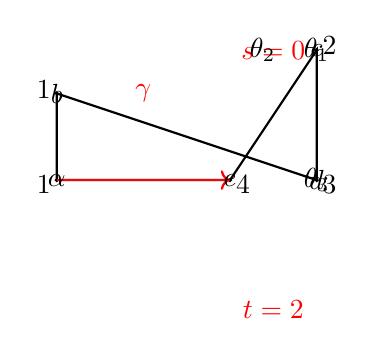
\begin{tikzpicture}[scale=0.55]
        \filldraw (0,0) circle (1pt);
        \node at (-0.3,-0.1) {$1$};
        \filldraw (4,0) circle (1pt);
        \node at (4.3,-0.1) {$4$};
        \filldraw (6,3) circle (1pt);
        \node at (6.3,3.1) {$2$};
        \filldraw (6,0) circle (1pt);
        \node at (6.3,-0.1) {$3$};
        \filldraw (0,2) circle (1pt);
        \node at (-0.3,2.1) {$1$};
        
        \draw[thick] (0,0) -- (4,0) -- (6,3) -- (6,0) -- (0,2) -- cycle;
        
        \draw[red, thick, ->] (0,0) -- (4,0);
        \node at (2,2) {\textcolor{red}{$\gamma$}};
        
        \node at (5,3) {\textcolor{red}{$s = 0$}};
        \node at (5,-3) {\textcolor{red}{$t = 2$}};
        
        \node at (6,0) {\textcolor{black}{$\theta_3$}};
        \node at (6,3) {\textcolor{black}{$\theta_1$}};
        \node at (4.75,3) {\textcolor{black}{$\theta_2$}};
        
        \node at (0,0) {\textcolor{black}{$\alpha$}};
        \node at (0,2) {\textcolor{black}{$b$}};
        \node at (6,3) {\textcolor{black}{$c$}};
        \node at (6,0) {\textcolor{black}{$d$}};
        
        \node at (4,0) {\textcolor{black}{$e$}};
        
    \end{tikzpicture}
    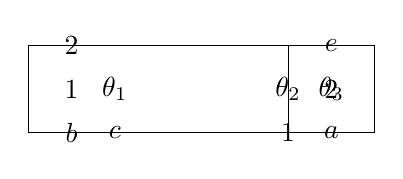
\begin{tikzpicture}[scale=0.55]
        \draw (0,0) rectangle (6,2);
        \draw (6,0) rectangle (8,2);
        
        \node at (1,1) {\textcolor{black}{$1$}};
        \node at (7,1) {\textcolor{black}{$2$}};
        
        \node at (1,0) {\textcolor{black}{$b$}};
        \node at (7,0) {\textcolor{black}{$a$}};
        
        \node at (1,2) {\textcolor{black}{$2$}};
        \node at (7,2) {\textcolor{black}{$e$}};
        
        \node at (2,0) {\textcolor{black}{$c$}};
        \node at (6,0) {\textcolor{black}{$1$}};
        
        \node at (2,1) {\textcolor{black}{$\theta_1$}};
        \node at (6,1) {\textcolor{black}{$\theta_2$}};
        \node at (7,1) {\textcolor{black}{$\theta_3$}};
    \end{tikzpicture}
    \caption{A triangulation of the pentagon with default orientation, and the snake graph of the longest arc $\gamma$ with source $s$ and target $t$ on the right.}
    \label{fig:pentagon-triangulation}
\end{figure}

\end{document}